\documentclass[../main.tex]{subfiles}
\begin{document}

\chapter{Integrative approaches for large-scale transcriptome-wide 
association studies, or: A test for significant \cis genetic correlation 
between expression and traits}
\labch{gusev2016}

\begin{external_abstract}{title=Abstract}
Many genetic variants influence complex traits by modulating gene 
expression, thus altering the abundance of one or multiple proteins. 
Here we introduce a powerful strategy that integrates gene expression 
measurements with summary association statistics from large-scale 
genome-wide association studies (GWAS) to identify genes whose 
cis-regulated expression is associated with complex traits. We leverage 
expression imputation from genetic data to perform a transcriptome-wide 
association study (TWAS) to identify significant expression-trait 
associations. We applied our approaches to expression data from blood 
and adipose tissue measured in \char`\~3,000 individuals overall. We 
imputed gene expression into GWAS data from over 900,000 phenotype 
measurements to identify 69 new genes significantly associated with 
obesity-related traits (BMI, lipids and height). Many of these genes are 
associated with relevant phenotypes in the Hybrid Mouse Diversity Panel. 
Our results showcase the power of integrating genotype, gene expression 
and phenotype to gain insights into the genetic basis of complex traits.
\end{external_abstract}

\section{Introduction}

The \textit{rationale} that lies behind the association of gene 
expression to phenotype is that many genetic variants influence traits 
by altering the regulation of the expression of some genes. Despite the 
strength of this argument, publications of studies in which both 
transcriptomic and phenotypic data are investigated simultaneously lag 
behind those of simple GWAS studies, for at least two reasons: first, 
although the cost of sequencing nucleic acids has been sharply 
decreasing for over a decade (\reffig{sequencingcost}), it can become 
quite an expensive technology if applied to cohorts of tens of thousand 
samples, such as those of a typical modern GWAS; secondly, every tissue 
shows a different pattern of expressed genes, and to choose the right 
tissue to analyse for each phenotype is not always a trivial matter.

\begin{marginfigure}[-4cm]
	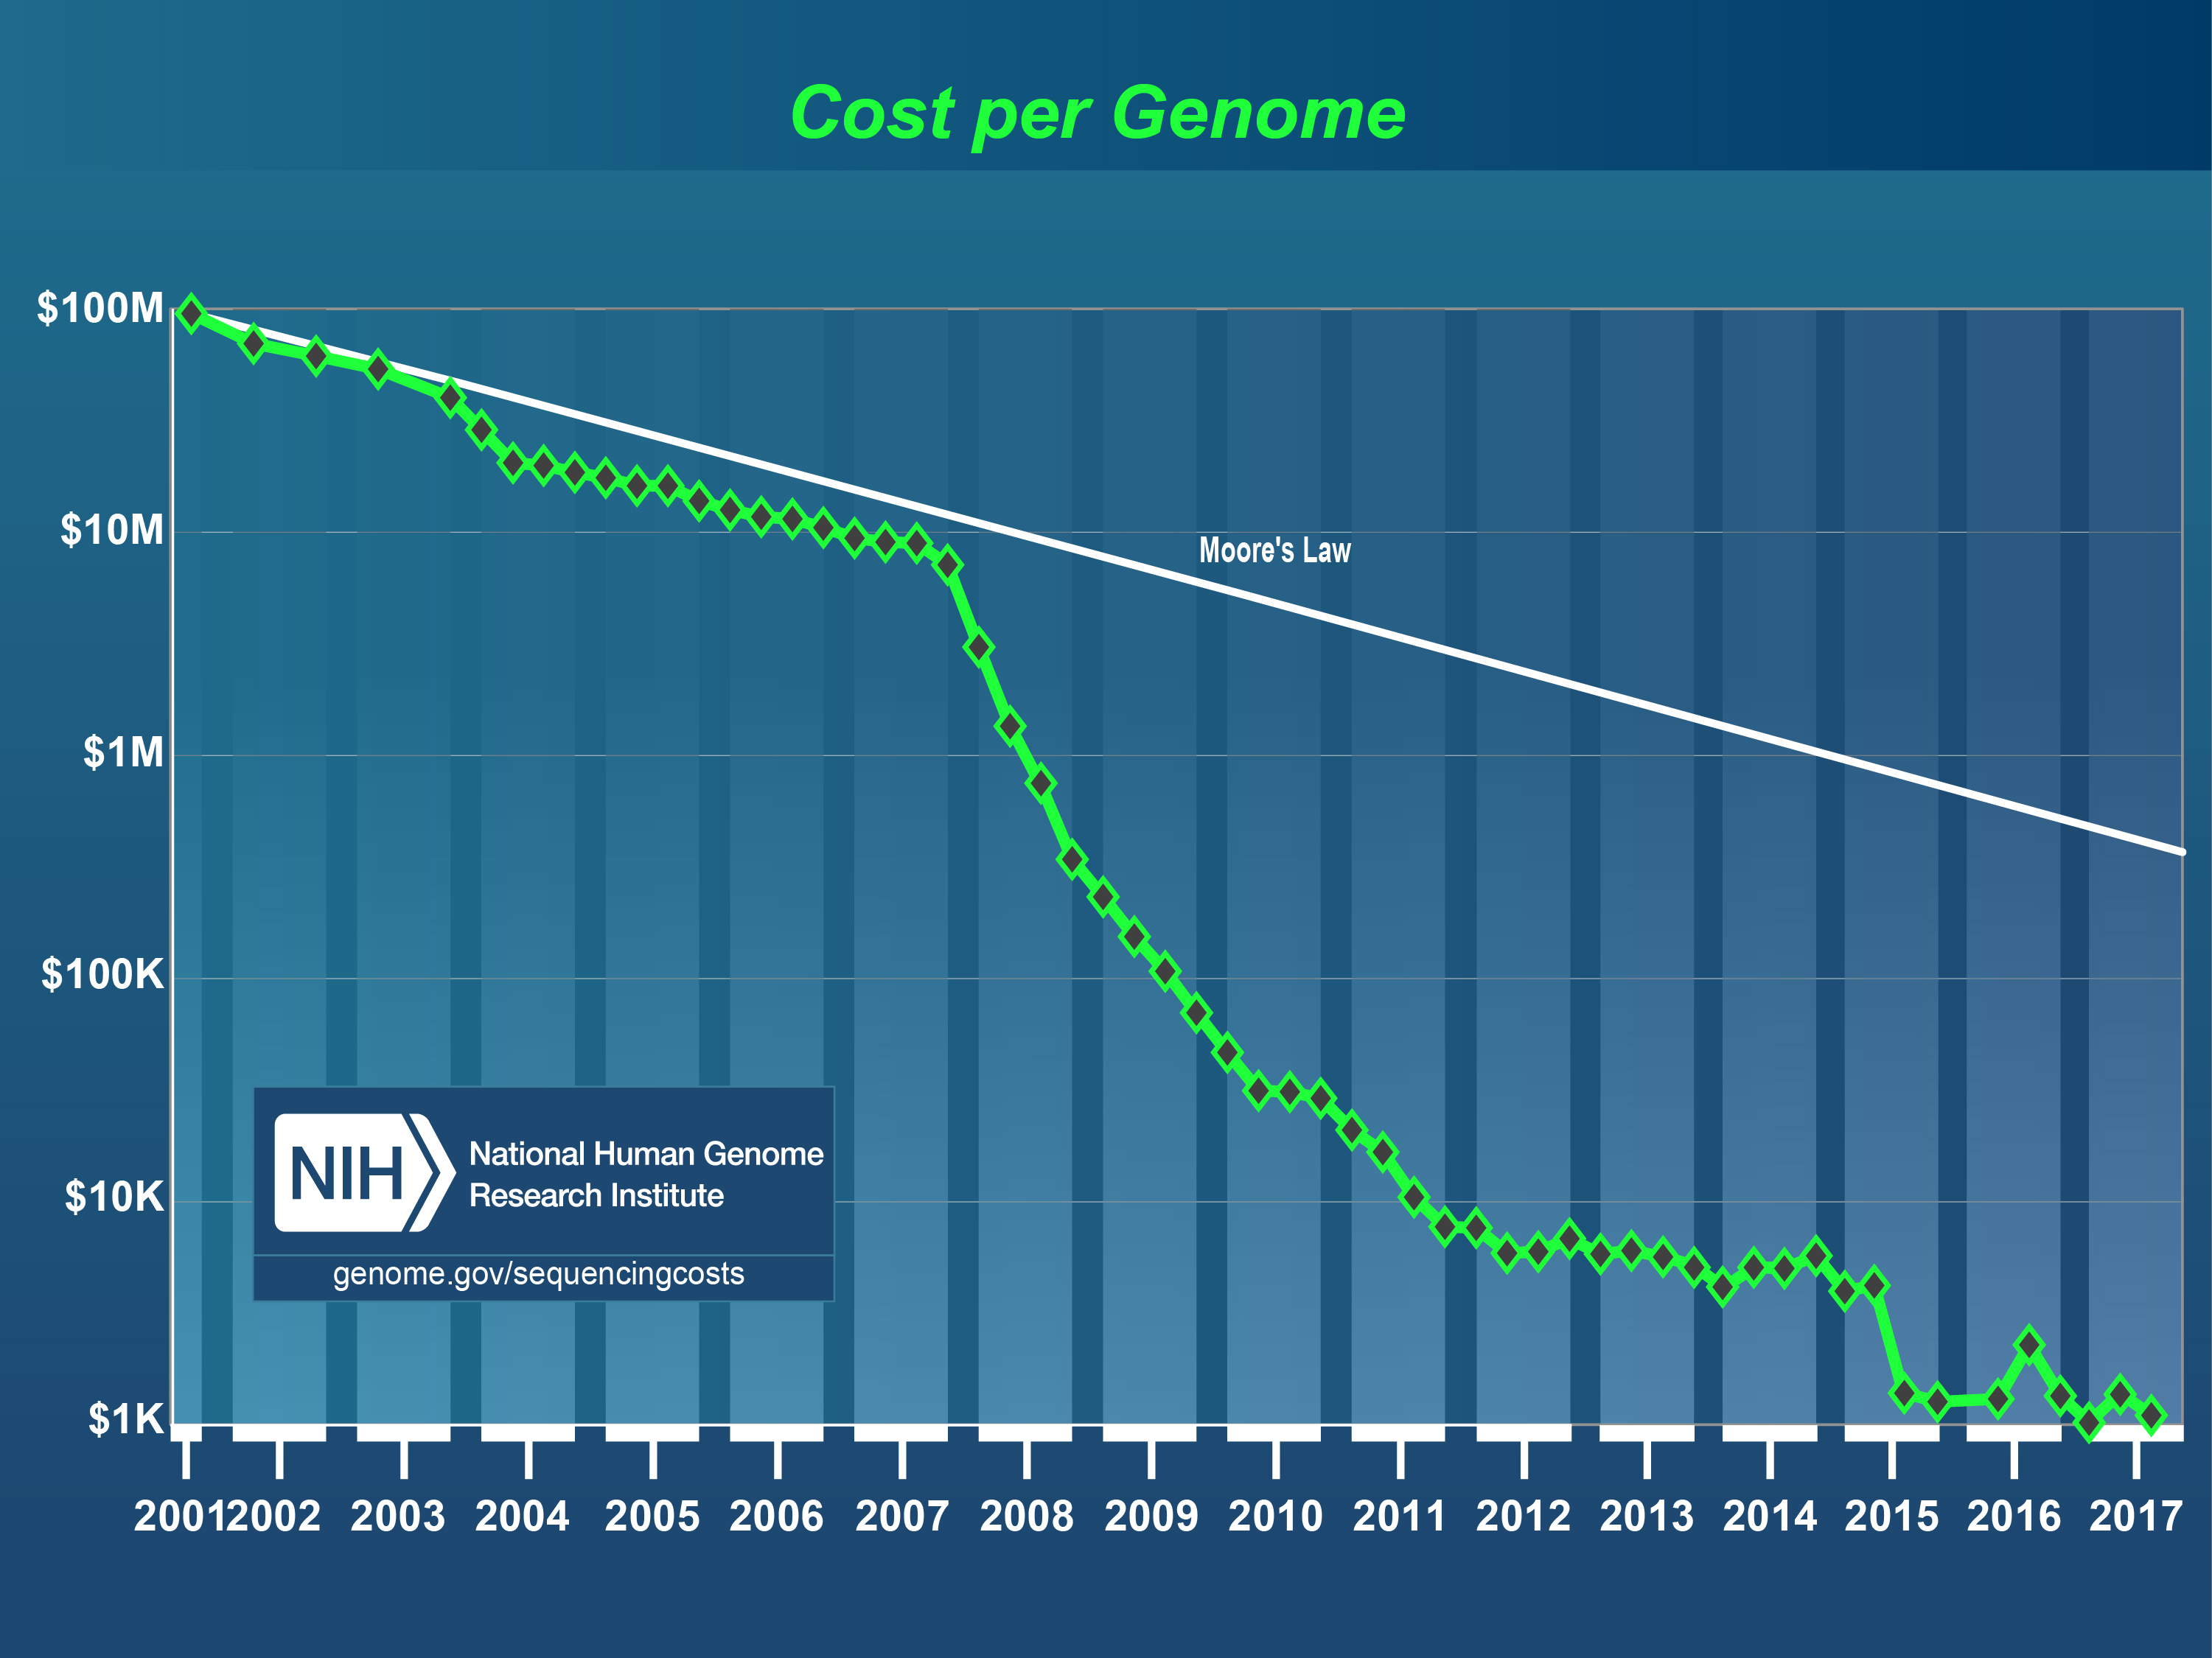
\includegraphics{sequencingcost}
	\caption[Sequencing cost over time]{The decrease in the cost of 
	genome sequencing; the same technology is used to sequence RNA. 
	\url{https://www.genome.gov/sequencingcosts/}}
	\labfig{sequencingcost}
\end{marginfigure}

In order to harness the plethora of data available from existing 
large-cohort GWAS studies, which, due to their great sample size, have 
the statistical power to find association even for rare and small-effect 
variants, many new methods are being developed. One of such methods is 
PrediXcan, with which we dealt in the previous section, but it is by no 
means the only one. In particular, in 2016 a new approach has been 
proposed which does not need individual-level data, but only summary 
association statistics\sidenote[][0cm]{By summary association statistics 
we mean, for instance, the effect size of all the SNPs} from a GWAS, 
which is an important advantage since, normally, only the summary-level 
data of a study is publicly available due to privacy concerns.

In essence, this approach is not different from PrediXcan: first, a 
linear regression model finds the correlation between each SNP and gene 
expression and accordingly assigns a weight to the SNP \todo{taking into 
account LD: gamazon used elastic net to prune correlated predictors}; 
next, the SNPs weights are used to impute the \cis genetic component of 
expression; finally, the imputed gene expression is tested for an 
association \todo{through correlation} with a complex trait.

\begin{figure}
	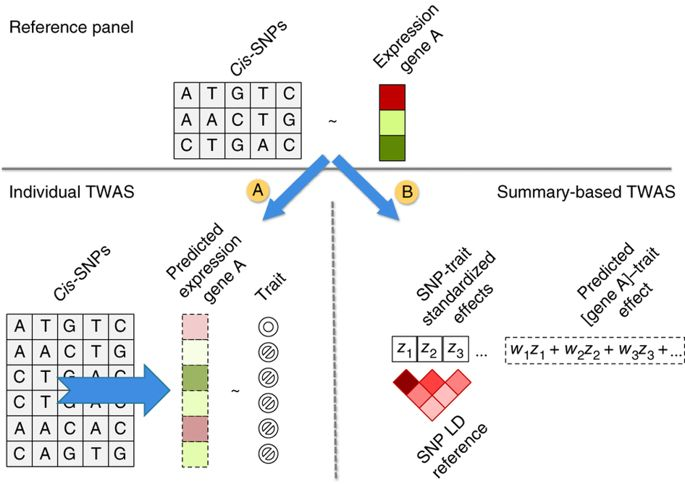
\includegraphics{gusev2016/1-TWAS_schematic}
	\caption{}
	\labfig{gusev2016/1}
\end{figure}

Nevertheless, there are some relevant points in this new method, 
relative to PrediXcan: its being based on summary association statistics 
greatly increases the effective sample size, because the method can in 
principle be applied to any GWA study; moreover, the authors emphasise 
the robustness of their approach, for its focus is on the genetic 
component of expression only, therefore it is guaranteed that the 
association between expression and trait is ultimately due to genetic 
factors.\todo{it doesn't mean it is robust}

Indeed, there are several ways in which genomic variation can be related 
to gene expression and phenotypic variation.\todo{approfondire}

\begin{marginfigure}[-2cm]
	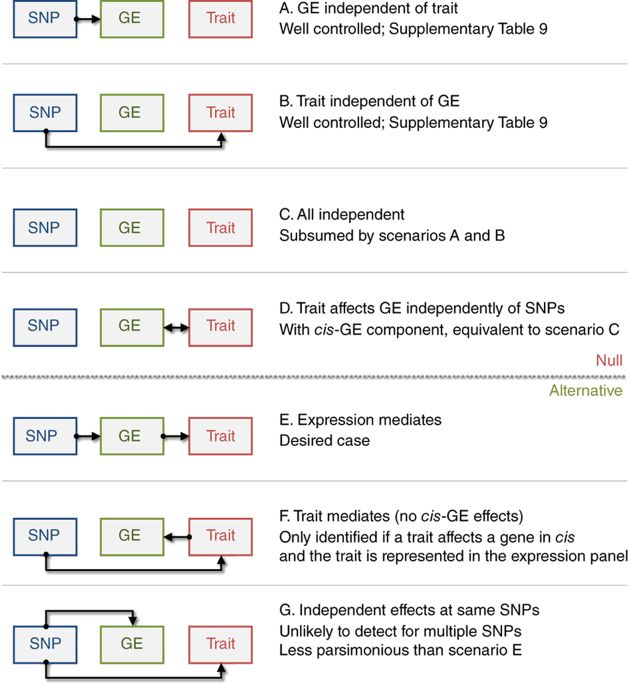
\includegraphics{gusev2016/2-causality_models}
	\caption{}
	\labfig{gusev2016/2}
\end{marginfigure}

Technically, here the weight of a SNP is its effect size.

The models were trained on about 3,000 individuals whose expression data 
from blood and adipose tissues, as well as genotype data, were 
available. With the help of a simulated dataset, they compared their 
approch with others previously proposed, showing that theirs is a 
significant improvement. Moreover, they reanalysed an existing dataset 
of a small-cohort lipid GWAS, finding that most of the novel 
associations they obtained had been previously reported in a 
large-cohort GWAS, and implying that their method is statistically more 
powerful than SNP-based approaches. Finally, they applied their method 

additional sections: heritability and genetic heterogeneity.

\section{Training of the expression model}

The accuracy of the prediction of a gene's expression cannot be greater 
than the heritability\todo{heritability: where to put this discussion?} 
of the expression of that gene itself. For instance, let us consider 
height\sidenote[][0cm]{Height is a typical, quantitative trait, and we 
choose to base our discussion on it because it is also quite easy to 
visualise; nevertheless, everything is still valid for gene expression, 
which is another quantitative trait.} and suppose that this trait is 
normally-distributed in the population. If every individual has the same 
alleles at the same height-associated loci, the genetic variance in that 
population will be 0, and the heritability for height would consequently 
be 0 as well. In such circumstances, it is not possible to predict 
height using the \cis-genetic component of gene expression, because 
there is no such component: the differences in the individuals' heights 
depend only upon the environment. Theoretically, the effect of the 
environment could be decomposed in a deterministic one and a random 
component, and the deterministic one could be associated with the trait; 
however, it is notoriously difficult to quantitatively measure the 
effect of the environment, especially outside of the laboratory. On the 
other hand, if the trait has an $h^2$ of 1, its manifestation can be 
predicted from the genotype with arbitrary accuracy.\todo{there are 
still effects of chance}

In order to predict a quantitative trait from the genotype of the 
individuals, a sample for which both gene expression and genotype data 
are present is necessary. The authors collected these data from three 
data sets: METISM, YFS and NTR.\todo{describe data sets}

From such individuals' data, the heritability of the expression of each 
gene was computed. For each gene, two heritability measures were 
estimated, \cis- and \trans- heritability, labelled $h_{g,cis}^2$ and 
$h_{g,trans}^2$; \cis-heritability refers to the proportion of variance 
in gene expression that is imputable to variance in loci up to 1Mb from 
the gene, whereas \trans-heritability is the proportion of variance in 
gene expression explained by the rest of the loci. Since on average any 
two non-related individuals differ at 0.1\% of loci \todo{citation 1000 
genomes}, in order to estimate \trans variance a very large sample size 
is needed, far larger than the 3,000 individuals used in this study, and 
this is the reason why estimates of \trans-heritability are close to 0. 
All subsequent analysis were based on the 6,924 \cis-heritable genes 
(\reffig{gusev2016/3}). Restricting the analysis to \cis-SNPs greatly 
increases the statistical power of the study, for the number of 
predictors of gene expression is quite small; as previously explained, 
the multiple testing burden is also decreased.

\begin{marginfigure}[-4cm]
	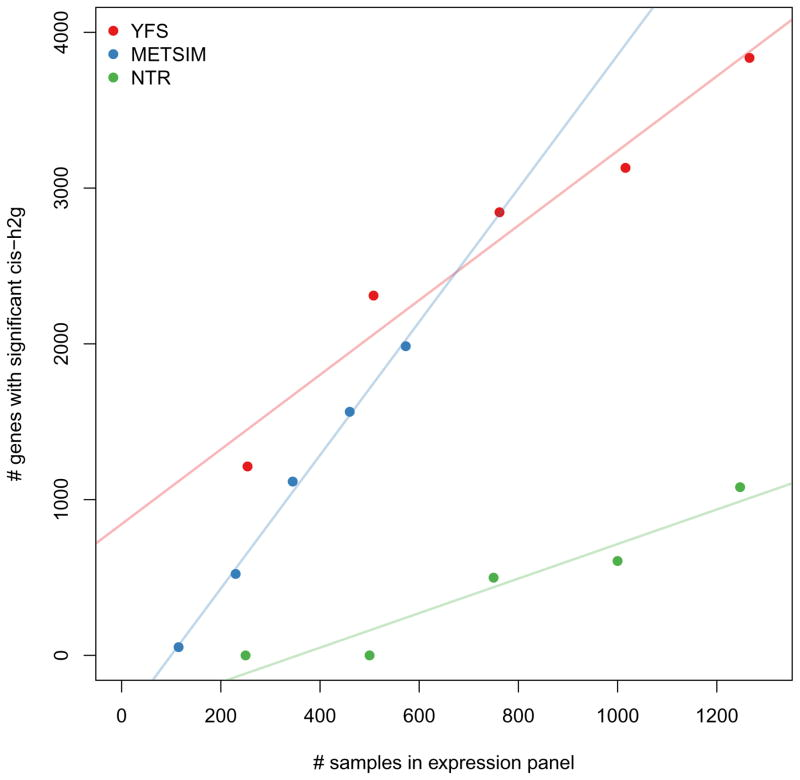
\includegraphics{gusev2016/3-heritable_genes}
	\caption{The 6,924 heritable genes, distributed according to their 
origin}
	\labfig{gusev2016/3}
\end{marginfigure}

\begin{figure}
	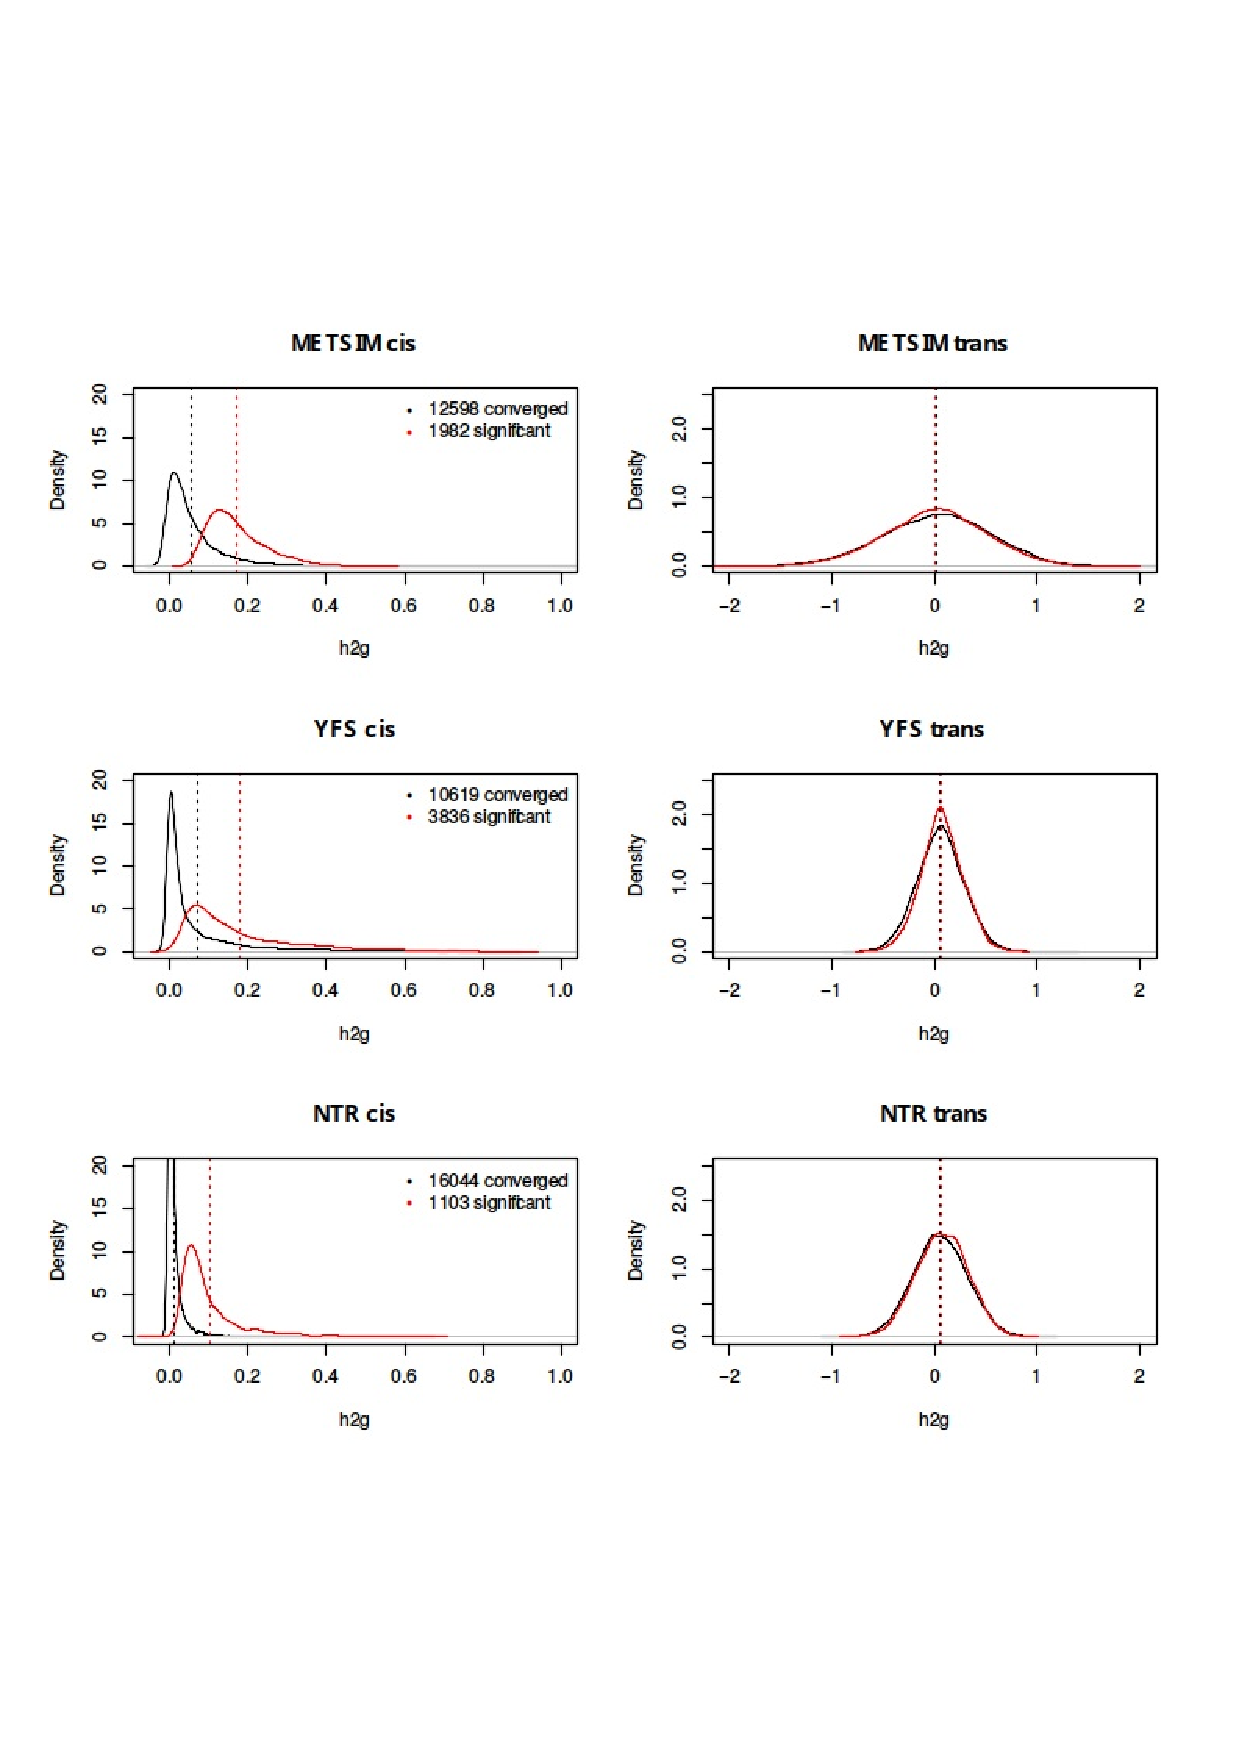
\includegraphics{gusev2016/S1-heritability_distribution}
	\caption{Heritability distribution.}
	\labfig{gusev2016/S1}
\end{figure}

Having computed heritability, a statistical model could be trained to 
predict gene expression from genotype data. Two different models, 
starting with the \cis-SNPs, were employed: the first was a best linear 
unbiased model (BLUP) and the second a Bayesian model (BSLMM); the 
performance of each model was evaluated by cross-validation. Moreover, 
these two models were compared to the predictions of gene expression 
made from the best cis-eQTL. The Bayesian model was the best one.

\begin{figure}
	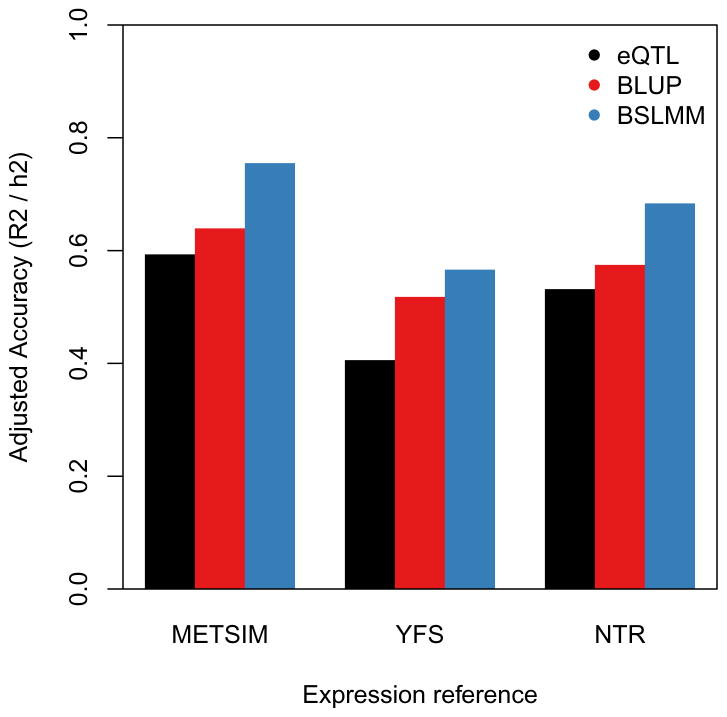
\includegraphics{gusev2016/4-prediction_accuracy_comparison}
	\caption{BSLMM performs better}
	\labfig{gusev2016/4}
\end{figure}

\todo{What is the trick? every gene is averaged from all the people? I 
think the trick is that the weigh of a snp is its effect size.}

\section{Simulations}

For comparison purposes, the authors built an array of simulated data 
sets, each modeling a possible scenario (1 causal variant, 5\% causal or 
10\% causal), and performed TWAS, GWAS and eGWAS on them. On the whole, 
TWAS performance was comparable to the others' when the number of causal 
variants was small, but it was the best at associating multiple causal 
variants to the trait.

\begin{figure}
	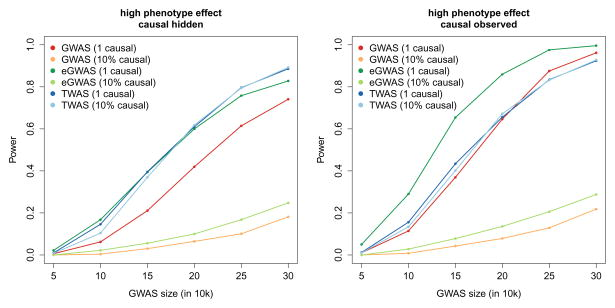
\includegraphics{gusev2016/5-association_power}
	\caption{Powerful!}
	\labfig{gusev2016/5}
\end{figure}

I am skipping three paragraphs where they 1) compare TWAS with coloc 
2) and another thing; 3) investigate on the effect of a larger sample 
   size for expression.

\section{small-cohort GWAS}

In the previous section, the authors showed that predicting gene 
expression from the summary-level statistics of a GWAS is feasible; here 
they show that associating gene expression to the trait is useful. In 
other words, they split their approach in two parts and validated them 
separately.

A previous study had reported all the 697 known loci associated to 
height. For each locus, Gusev etal selected a single causal gene 
according to three different strategies:

The third strategy seems a bit circular: they select the best twas gene, 
and then associate its expression with the trait; but is the best gene 
not found already by its association with the trait?

I give up this section. I think it tries to say that performing twas on 
summary level or directly on real expression is identical.

\section{900000 phenotypes}

One of the most innovative features of this approach is its broad 
applicability. Indeed, its potential was unleashed on three GWAS which 
account for over 900,000 phenotype measurements of obesity-related 
traits\sidenote[][0cm]{Lipid measures (high-density lipoproteins [HDL] 
cholesterol, low-density lipoprotein [LDL] cholesterol, total 
cholesterol [TC], and triglycerides [TG]); height; and BMI}. They first 
imputed gene expression for the 6,924 genes whose expression is 
heritable, then associated such imputed expression to the trait, 
correcting for the multiple testing, and finding 665 significant 
gene-trait associations, 69 of which genes did not overlap any SNP which 
was reported by the original GWA studies.

\enquote{Averaging over the novel genes, the Z2 statistics from TWAS 
were 1.5x higher than the strongest eQTL SNP for the same gene(though 
this may be slightly inflated due to winner’s curse).}

They used a permutation test\todo{come back here when the methods are 
understood}. Allelic heterogeneity strikes back.\todo{put a subsection 
on heritability in gamazon and a subsection on heretogeneity here}

Paragraph on the contribution to heritability of the associations. I 
think they say that if a gene is associated, it contributes to the 
heritability.

Paragraph where they used muther and another thing to train the 
expression models. They still found many of the associations. (only the 
training changes, the three gwas summary are the same.)

Those 69 novel associations are the most interesting ones, therefore 
they were the focus of a functional analysis: on the one hand, their 
presence was sought in the Hybrid Mouse Diversity Panel (HMDP), which 
collects obesity-related phenotypes; on the other, tissue-specific 
enrichments of these genes was evaluated. Many of the 69 genes were 
indeed present and they were associated with an obesity-related trait. 
Moreover, the enrichment analysis, performed with DEPICT, showed that 
the novel genes were specific of hypothalamus and neurosecretory 
systems, which is consistent with recent discoveries on 
obesity.\todo{cite obesity papers}

\section{Methods}

\subsection{Heritability computation}

\end{document}
